\documentclass[a4paper,12pt]{article}

\usepackage{../../../mypackages}

\usepackage{pgfplots}
    \pgfplotsset{
    compat=1.11,
  }

\usetikzlibrary{shapes,arrows,babel}
\tikzstyle{box}=[minimum size = 0.1cm, rectangle, draw=black, fill=gray]
  

\newcommand{\ans}[3]{
  % 1st argument is the answer
  % 2nd argument is the # of lines for the blank answer
  % 3rd argument is whether the lines should be filled with blanks or dots
  \ifthenelse{\equal{\WITH_CORRECTION}{NO}}{%
    \ifthenelse{\equal{#3}{TRUE}}{
      \foreach \i in {1,...,#2} {%
      \noindent\makebox[\linewidth]{\dotfill}%
      \ifnum\i<#2\\[0.5em] \fi
      }
    }
    {% FALSE statement of the IF for dots
    \foreach \i in {1,...,#2} {%
    \noindent\makebox[\linewidth]{} % Leaves the box empty
    \ifnum\i<#2\\[0.5em] \fi
    }
    }
  }{% If \WITH_CORRECTION is YES, print the answer
  \noindent\parbox{\linewidth}{#1}
  }
}

\def\WITH_CORRECTION{YES}


\begin{document}

\title{Fonctions - Rappels de 2nde}
\author{N. Bancel}


\sloppy  % This will apply the sloppy setting to the entire document.
\maketitle

\section{Vocabulaire des fonctions - Fonctions affines}

\begin{enumerate}
  \item A chaque nombre réel \(x\) d'un intervalle \(I\), une fonction \(f\) associe un nombre réel et un seul que l'on note \(f(x)\). Qu'est ce qu'une image ? Qu'est-ce que l'ensemble de définition ? Qu'est qu'un antécédent ? \par
  \ans{
    \begin{minipage}{0.5\textwidth}
    \begin{itemize}
      \item[$\bullet$] \(f(x)\) est \textbf{l'image} de \(x\) par la fonction \(f\)
      \item[$\bullet$] \(I\) est \textbf{l'ensemble de définition} de \(f\)
      \item[$\bullet$] Lorsque \(y = f(x)\), on dit que le nombre \(x\) est un \textbf{antécédent} du nombre \(y\) par la fonction \(f\)
    \end{itemize}
    \end{minipage}%
    \begin{minipage}{0.5\textwidth}
    \centering
    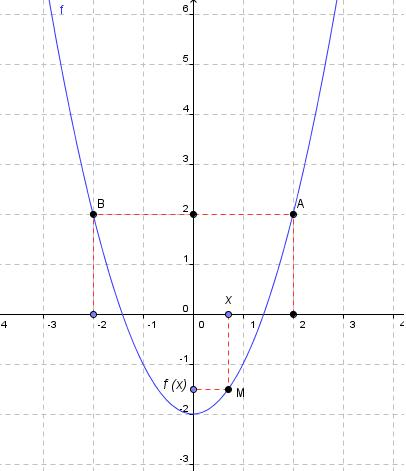
\includegraphics[width=0.5\textwidth]{image_antecedent.jpg}
    \end{minipage}
    Dans la figure ci-dessus : 
    \begin{itemize}
      \item[$\bullet$] Si M a pour abscisse \(x\), alors son ordonnée est \(f(x)\).
      \item[$\bullet$] A a pour coordonnées (2 ; 2), donc \(f(2) = 2\), donc \textbf{l’image de 2 par \(f\) est 2}.
      \item[$\bullet$] B a pour coordonnées (-2 ; 2), donc \(f(-2) = 2\) donc \textbf{l’image de -2 par \(f\) est 2}.
      \item[$\bullet$] Les \textbf{antécédents} de 2 par la fonction f sont -2 et 2.
    \end{itemize}
    }{6}{FALSE}
    \item A partir du graphique ci-dessous, résoudre graphiquement l'équation \(f(x) = k\) \par
    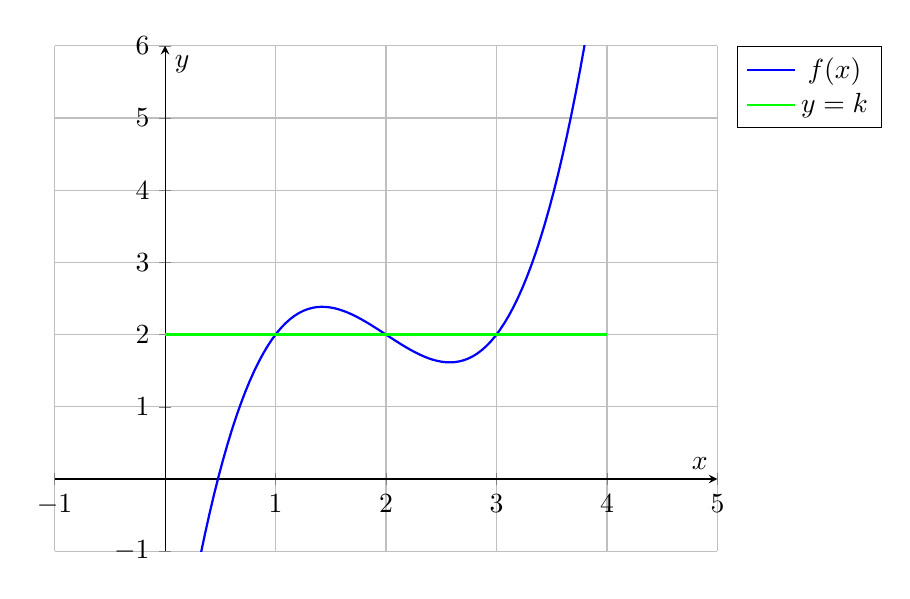
\begin{tikzpicture}
      \begin{axis}[
          axis lines = middle,
          xlabel = {$x$},
          ylabel = {$y$},
          xmin=-1, xmax=5,
          ymin=-1, ymax=6,
          domain=0:4,
          samples=100,
          legend pos=outer north east,
          grid=major,
          width=10cm, height=8cm,
      ]
      % Plot f(x) = (x-1)*(x-2)*(x-3) + 2
      \addplot[color=blue, thick] {(x-1)*(x-2)*(x-3) + 2};
      \addlegendentry{$f(x)$}
      
      % Plot y = k
      \addplot[color=green, thick] {2};
      \addlegendentry{$y = k$}
      \end{axis}
      \end{tikzpicture} \par 
  
    \ans{
      Hello this is a test for answer macro

      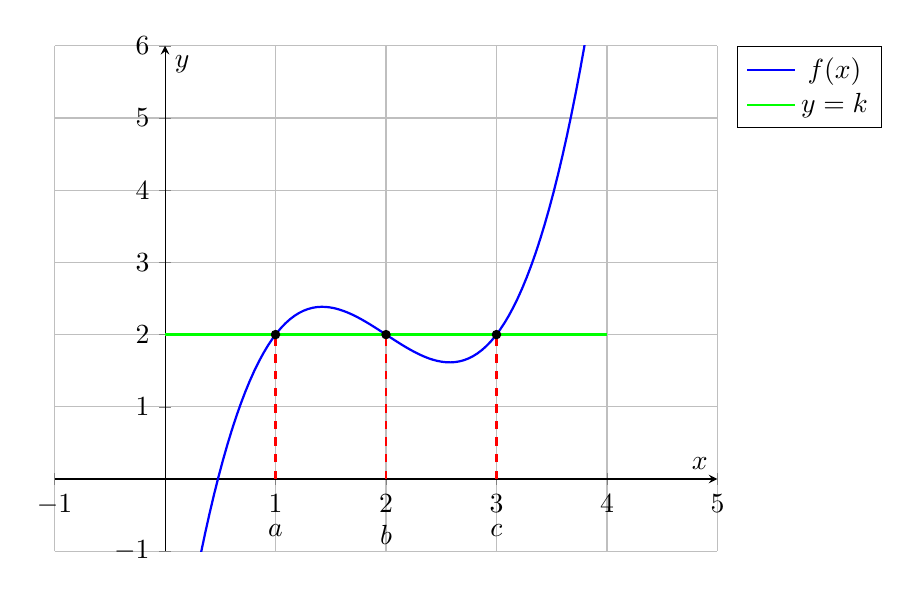
\begin{tikzpicture}
        \begin{axis}[
            axis lines = middle,
            xlabel = {$x$},
            ylabel = {$y$},
            xmin=-1, xmax=5,
            ymin=-1, ymax=6,
            domain=0:4,
            samples=100,
            legend pos=outer north east,
            grid=major,
            width=10cm, height=8cm,
        ]
        % Plot f(x) = (x-1)*(x-2)*(x-3) + 2
        \addplot[color=blue, thick] {(x-1)*(x-2)*(x-3) + 2};
        \addlegendentry{$f(x)$}
        
        % Plot y = k
        \addplot[color=green, thick] {2};
        \addlegendentry{$y = k$}
        
        % Mark the solutions
        \addplot[mark=*, mark size=1.5pt, color=black] coordinates {(1, 2)};
        \addplot[mark=*, mark size=1.5pt, color=black] coordinates {(2, 2)};
        \addplot[mark=*, mark size=1.5pt, color=black] coordinates {(3, 2)};
    
        \addplot[red, dashed, thick]
                coordinates {(1, 0) (1, 2)};
        \addplot[red, dashed, thick]
                coordinates {(2, 0) (2, 2)};
        \addplot[red, dashed, thick]
                coordinates {(3, 0) (3, 2)};
        
        % Labels for the solutions
        \node at (axis cs: 1,-0.5) [anchor=north] {$a$};
        \node at (axis cs: 2,-0.5) [anchor=north] {$b$};
        \node at (axis cs: 3,-0.5) [anchor=north] {$c$};
        
        \end{axis}
        \end{tikzpicture}
    }{6}{FALSE}

    \end{enumerate}
  \end{document}
